\documentclass{report}

\usepackage{booktabs}
\usepackage{url}
\usepackage{cite}
\usepackage[version=4]{mhchem}
\usepackage{graphicx}
\usepackage{subfigure}
\usepackage[a4paper,top=2cm,bottom=2cm,right=3cm,left=3cm,marginparwidth=1.75cm]{geometry}
\usepackage{amsmath}

\title{3CL SARS-CoV-2 3CL Protease Analyzing}
\author{Yan Haoming}
\date{September 27, 2024}


\begin{document}
\maketitle
\chapter{Protein Purification}
\section{\textit{E.coli} Lysis: Homogenizer}
\subsection{Materials}
\begin{itemize}
    \item Buffer Lysis
    \begin{itemize}
        \item PBS (Phosphate Buffered Saline: \ce{HPO_4^2- / H2PO_4-}): 20 mM (pH=7.3)
        \item \ce{NaCl}: 500 mM
        \item Imidazole: 10 mM
        \item DTT (Dithiothreitol: Reducing Agent): 1 mM
        \item PMSF (Phenylmethanesulfonyl Fluoride: Serine Protease Inhibitor): 1 mM
    \end{itemize}
\end{itemize}
\subsection{Experimental Procedure}
\begin{itemize}
    \item Stir the buffer lysis containing \textit{E.coli} until without obvious lumps and precipitates in an ice bath.
    \item Filter the mixture (50 mL) by gauze and then pour into the \textbf{homogenizer}\cite{Homogenization} with 10 mL \ce{H2O} following the below settings:
    \begin{itemize}
        \item Raise the pressure to 1,000 bar for 2 minutes.
        \item Pause 1 minute.
        \item Repeat the cycle 3 times.
    \end{itemize}
    \item Centrifugate the liquid at 14,000 rpm for 30 minutes.
    \item Strain the product through a filter (0.45 $\mu$m) into a graduated cylinder.
\end{itemize}
\section{Purification: Column Chromatography}

\subsection{Materials}
\begin{itemize}
    \item Buffer A
    \begin{itemize}
        \item PBS (Phosphate Buffered Saline: \ce{HPO_4^2- / H2PO_4-}): 20 mM (pH=7.3)
        \item \ce{NaCl}: 500 mM
        \item Imidazole: \textbf{10 mM}
    \end{itemize}
    \item Buffer B
    \begin{itemize}
        \item PBS (Phosphate Buffered Saline: \ce{HPO_4^2- / H2PO_4-}): 20 mM (pH=7.3)
        \item \ce{NaCl}: 500 mM
        \item Imidazole: \textbf{500 mM}
    \end{itemize}
    \item Buffer C
    \begin{itemize}
        \item PBS (Phosphate Buffered Saline: \ce{HPO_4^2- / H2PO_4-}): 40 mM (pH=7.3)
        \item \ce{NaCl}: 100 mM
        \item EDTA: 1 mM
    \end{itemize}
\end{itemize}
\subsection{Affinity Chromatography: Immobilized \ce{Ni^2+} Metal Ion + His-tag}
\subsubsection{Experimental Procedure}
We purified 3CL protease fist by affinity chromatography.
Immobilized \ce{Ni^2+} ion had been attached to the column while His-tag (six histidine in the terminal of protein) had been fused with 3CL protease.

The \ce{Ni^2+} column has the capacity of 5 mL.
We washed the column before loading using buffer A and buffer B in turn (A(25 mL)-B(25 mL)-A(15 mL)-B(15 mL)-A(15 mL)) as shown in the blue curve in Figure \ref{Affinity Chromatography: UV Absorbance} and Figure \ref{Affinity Chromatography: Conductance}.
We set pressure difference ($\Delta P=0.3$ MPa) to be the control threshold with the pre-column pressure ($P_{pre}=0.5$ MPa).
The flow rate was set to be 1 mL/min for above operation.

Then we loaded 55 mL sample after lysis into the column with the flow velocity to be 2 mL/min.
After that, buffer A was constantly pumped into to column to elute impurities until the signal of UV absorbance went back near 0 mAU.
Once the eluting was complete, we started to raise the proportion of buffer B linearly to form a linear gradient.
The threshold to collect product was set to be 20 mAU.
The fraction collecting was performed automatically with the amount of 1.8 mL/tube.
Finally, we collected tubes from number 3 to number 8, totally $6\times1.8=10.8$ mL.

Condensation with centrifuging filtering and solvent changing was used condense 10.8 mL solution to nearly 1.5 mL.
The centrifuging was in 4$^\circ$C with the rotating speed of 3,500 rpm for 10 minutes.
In each turn, we decanted 5 mL solvent for the Gel-filtration Column to replace the buffer for \ce{Ni^2+} column containing lots of imidazole.

\subsubsection{Results}
The tracking of UV absorbance changing and conductance changing with varied buffer B proportion can be seen in Figure \ref{Affinity Chromatography: UV Absorbance} and Figure \ref{Affinity Chromatography: Conductance}.
The major peak in the middle of the Figure \ref{Affinity Chromatography: UV Absorbance} corresponds to the impurities (protein that has UV absorbance companied by nucleic acid).
Meanwhile the conductance drops down (Figure \ref{Affinity Chromatography: Conductance}) due the poor conductivity of protein compared with inorganic salts.

From the Fourth Column in Figure \ref{Results of SDS-PAGE} we can clearly see the effective purification produced by affinity chromatography compared with the lysis mixture in second and third column.

\begin{figure}
    \centering
    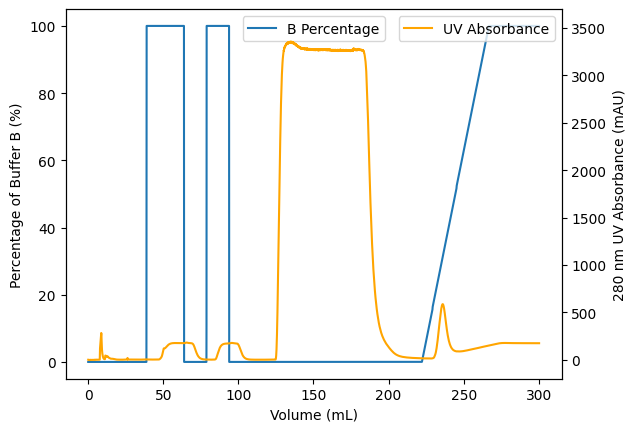
\includegraphics[width=0.6\linewidth]{../Figures/Affinity Column UV.png}
    \caption{Affinity Chromatography: UV Absorbance with Percentage of Buffer B}
    \label{Affinity Chromatography: UV Absorbance}
\end{figure}

\begin{figure}
    \centering
    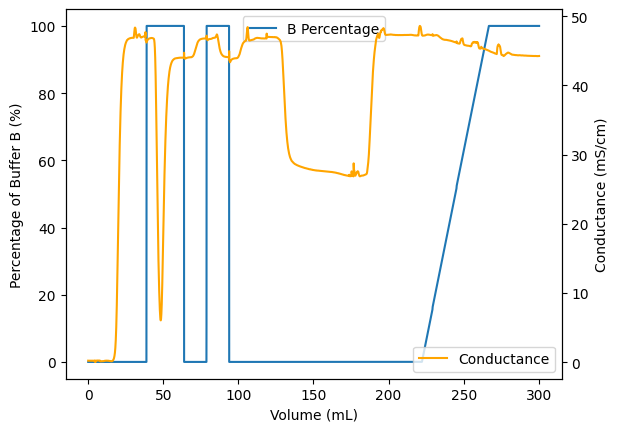
\includegraphics[width=0.6\linewidth]{../Figures/Affinity Column Conductance.png}
    \caption{Affinity Chromatography: Conductance with Percentage of Buffer B}
    \label{Affinity Chromatography: Conductance}
\end{figure}


\subsection{Gel-filtration Chromatography}
\subsubsection{Experimental Procedure}
The Gel-filtration Column has the capacity of 24 mL.
We set pressure difference ($\Delta P=1.8$ MPa) to be the control threshold with the pre-column pressure ($P_{pre}=5.0$ MPa).
Careful washing of the column and sample ring was performed.
As for the sample ring, 4 mL ultra-pure water with 4 mL buffer assay were used to expel the air.
The two direction of washing(up to down and vice versa) with careful injector operation was included to ensure any bubble would be excluded from the column.

The loading amount should be 500 $\mu$L with the concentration of 1 mg/mL.
To ensure the sample concentration to be around 1 mg/mL, we detected the concentration of the sample by nano drop.
The result was 6.737 Abs equivalent to $6.737\times1.07=7.21$ mg/mL.
That means around 70 $\mu$L concentrated protease was needed with 430 $\mu$L buffer assay.
However we enlarged the system by two fold which means diluting 140 $\mu$L concentrated protease with 860 $\mu$L buffer assay in case of failure.



We collected according to the UV absorbance as shown in Figure \ref{Gel-filtration Chromatography: UV absorbance with Conductace} and Figure \ref{Gel-filtration Chromatography: UV absorbance with Percentage of Buffer B}.
Then condensed the sample as previous process in affinity chromatography.

\begin{align}
    A &= \epsilon cl \\
    A &= 6.737\ Abs \\
    \epsilon &= 0.937\ \text{L/g}\cdot\text{cm} \\
    l &= 1\ \text{cm}\\
    c &\approx 7.21\ \text{mg/mL}=\frac{7.21\ \text{g/L}}{35\times 10^3 \text{g/mol}}=205.4\ \mu\text{M}    
\end{align}

\subsubsection{Results}
The effect can be seen in Figure \ref{Results of SDS-PAGE}.
Compared with the fourth column, the last column after gel-filtration chromatography does not show additional purification.
Probably, the solution had been purified to an extreme extend after affinity chromatography, which leads to the unobvious improvement.

\begin{figure}
    \centering
    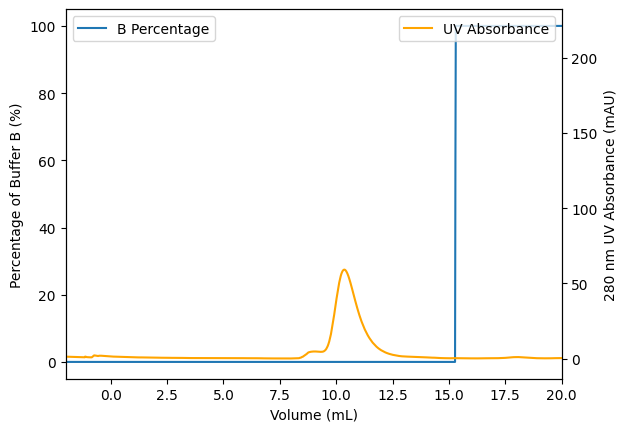
\includegraphics[width=0.6\linewidth]{../Figures/Filtration Column UV.png}
    \caption{Gel-filtration Chromatography: UV absorbance with Percentage of Buffer B}
    \label{Gel-filtration Chromatography: UV absorbance with Percentage of Buffer B}
\end{figure}

\begin{figure}
    \centering
    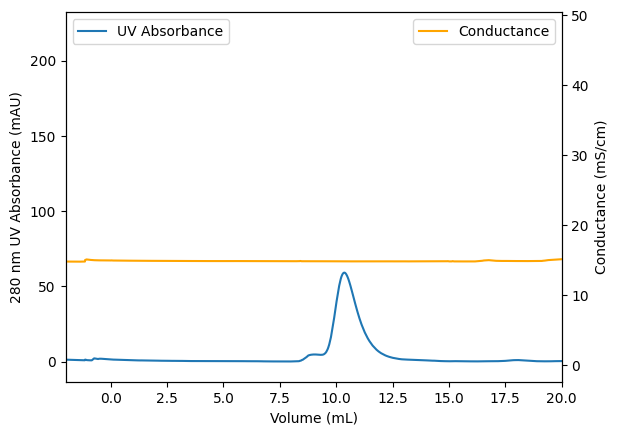
\includegraphics[width=0.6\linewidth]{../Figures/Filtration Column UV and Conductance.png}
    \caption{Gel-filtration Chromatography: UV absorbance with Conductance}
    \label{Gel-filtration Chromatography: UV absorbance with Conductace}
\end{figure}

\section{Analyzing: SDS-PAGE}
\begin{figure}
    \centering
    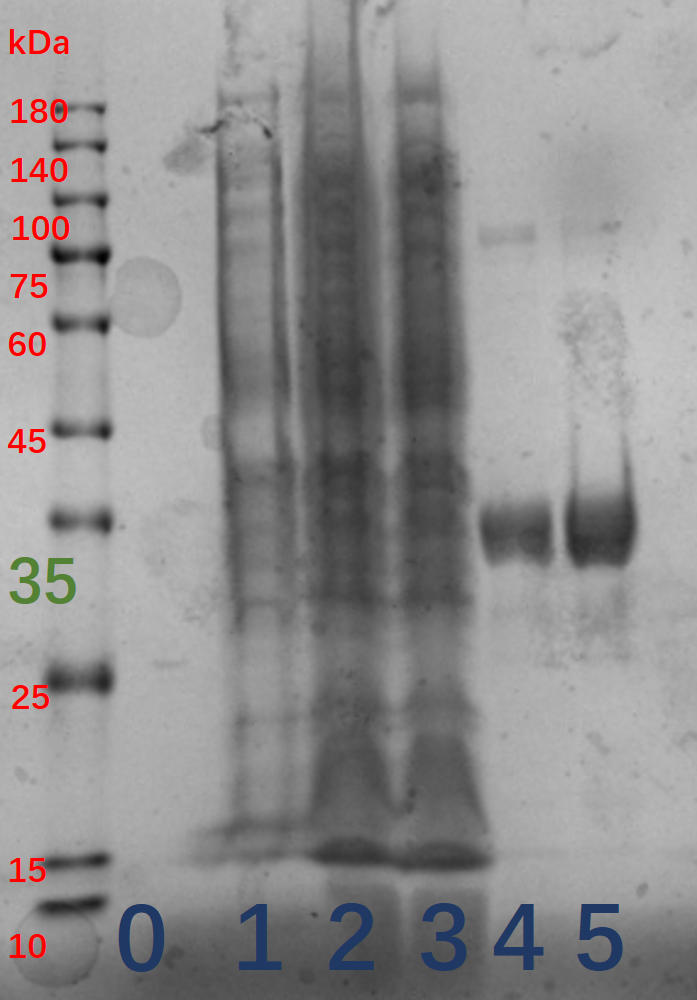
\includegraphics[width=0.7\linewidth]{../Figures/SDS-PAGE.png}
    \caption{Results of SDS-PAGE: The Second Column is the solution after lysis; The Third Column is from supernate; The Fourth Column is after affinity chromatography; The Last One is after gel-filtration chromatography. The First Column has the same composition as the second one just with additional loading buffer. The leftmost one is marker.}
    \label{Results of SDS-PAGE}
\end{figure}
\subsection{Experimental Procedure}
In this experiment, we used precast polyacrylamide gel.
However, we still need to prepare the buffer(500 mL) for electrophoresis by hands.

Four type of samples were prepared for SDS-PAGE to check the effect of protein purification.

\begin{itemize}
    \item No.1 \textit{E.coli} lysate
    \item No.2 Supernate of lysate after centrifuging
    \item No.3 Sample after affinity chromatography
    \item No.4 Sample after gel-filtration chromatography
\end{itemize}

In each well, we put 20 $\mu$L sample with 5 $\mu$L loading buffer except for No.3 which only left 8 $\mu$L.
To control the concentration in consistency, only 2 $\mu$L loading buffer was added to No.3.

We mixed the solution by \textbf{Vortex Genie 2} and centrifuge for instant.
Then heated at 94 $^\circ$C for 3 minutes.
Finally, loaded marker (2 $\mu$L) as well as the four types of sample (10 $\mu$L) into the polyacrylamide gel in sequence.

The electrophoresis apparatus was set at 150 V working for 38 minutes.

After electrophoresis, the gel was stained using Coomassie Brilliant Blue with heating in microwave oven for three times.
In each turn, the paint was heated until boiling.
\ce{H2O} plus acetic acid (3\%) was used to destain with the similar procedure in microwave oven.

\subsection{Results}
As shown in Figure \ref{Results of SDS-PAGE}, the effect of purification is obvious.
The most effective method should be affinity chromatography while other steps are also playing an important role in the whole process.
Besides, we can also figure out the molecular weight of 3CL protease which is near 35 kDa.

\chapter{Enzyme Kinetics}
\begin{figure}
    \centering
    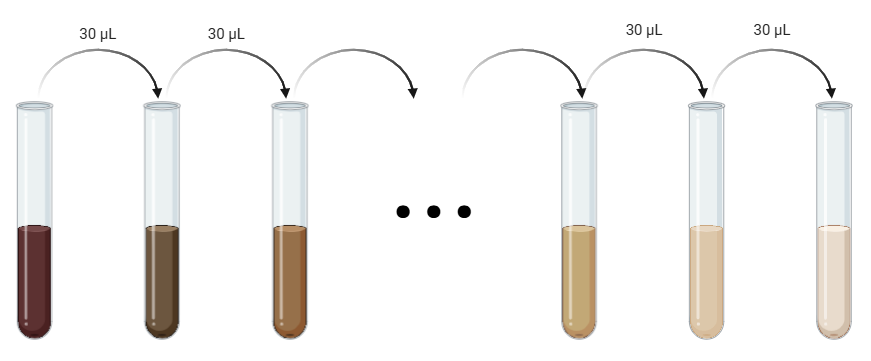
\includegraphics[width=0.7\linewidth]{../Figures/serial dilution.png}
    \caption{Serial Dilution of Inhibitor}
    \label{Serial Dilution of Inhibitor}
\end{figure}
\begin{figure}
    \centering
    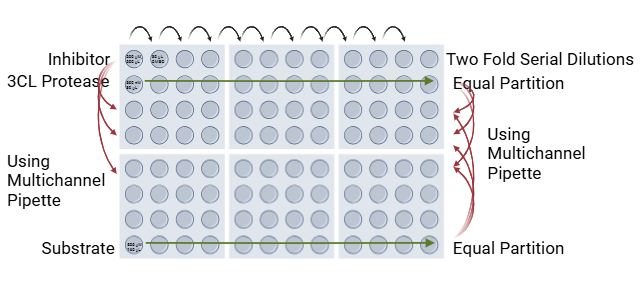
\includegraphics[width=1\linewidth]{../Figures/microplate.png}
    \caption{Solution Configuration in Microplate}
    \label{Inhibitor Solution Configuration in Microplate}
\end{figure}
The following experiments involve tedious configuration of solutions with different concentrations, including substrate, 3CL Protease (Enzyme), and inhibitor.
To summarize and visualize the complicated process of dilution, I have drawn the Figure \ref{Inhibitor Solution Configuration in Microplate}.
Generally speaking, we used \textbf{multichannel pipette} to transfer a whole row of solution to other three different rows because of the three independent parallel groups.
Before that, however, we must use \textbf{single-channel pipette} to adjust the concentration in one row.
The \textbf{two fold serial diluting}, as shown in Figure \ref{Serial Dilution of Inhibitor}, was used for inhibitor while substrate was diluted one by one differently as shown in Table \ref{Substrate Solution Configuration in Microplate}.

\section{Verifying Michaelis Menton Equation}
$$
E + S \rightleftharpoons ES \rightarrow E+P
$$

$$
V_0 =\frac{k_{cat}E_0[S]}{K_m+[S]}=\frac{V_{max}[S]}{K_m+[S]}
$$
% Table
\begin{table}
    \centering
    \caption{Substrate Solution Configuration in Microplate}
    
    \begin{tabular}{|c|c|c|c|c|c|c|c|c|} \hline
        Number of Sample&1&2&3&4&5&6&7&8 \\ \hline
        Substrate Concentration ($\mu$M)&500&750&1000&1250&1500&2000&2500&3000 \\ \hline
        DMSO Solvent ($\mu$L)& 9&8.5&8&7.5&7&6&5&4\\ \hline
        5000$\mu$M Concentrated Substrate ($\mu$L)&1&1.5&2&2.5&3&4&5&6 \\ \hline
    \end{tabular}
    \label{Substrate Solution Configuration in Microplate}
\end{table}

\subsection{Introduction}
The fluorescent substrate relates to \textbf{FRET}, which means the substrate will be fluorescent only when catalyzed by protease.
Specifically speaking, DABCYL plays the role of dark quencher\cite{Quencher} while the EDANS\cite{EDANS} as the donor of fluorescence.
The substrate (polypeptide) is stuck in the middle as shown in Figure \ref{Structure of Fluorescent Substrate}.
\begin{figure}
    \centering
    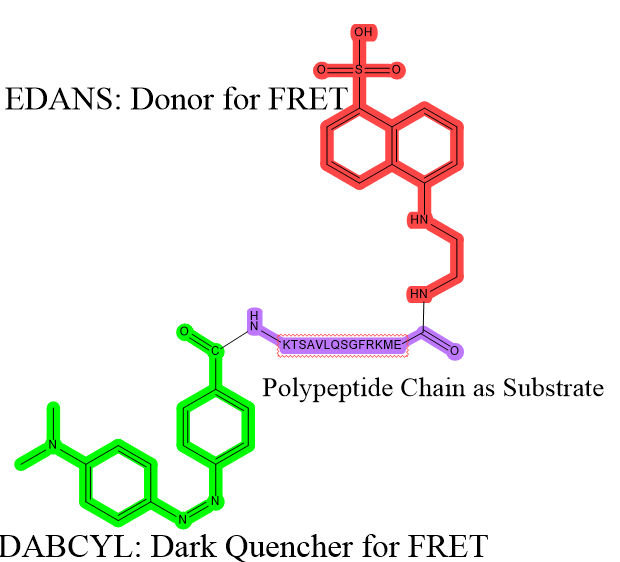
\includegraphics[width=0.5\linewidth]{../Figures/fluorescent substrate.png}
    \caption{Structure of Fluorescent Substrate}
    \label{Structure of Fluorescent Substrate}
\end{figure}

The overall consequence is that, when the substrate is consumed, then, it will show fluorescence.
Further process of reaction will lead to more intensive fluorescence which can be detected by \textbf{ELISA} in the unit of RFU.

\subsection{Experimental Procedure}

The independent variable in Michaelis Menton Equation is the concentration of substrate $[S]$.
Thus to verify the equation we must configure the substrate solution of different concentrations.
We started by dissolving 2 mg solid substrate into 192 $\mu$L DMSO solvent, which has the concentration of 5000 $\mu$M.
Then, we adjusted the ratio of DMSO and concentrated substrate to achieve 8 different concentrations of substrate solution, as shown in Table \ref{Substrate Solution Configuration in Microplate}.

The Composition of the System (100 $\mu$L):
\begin{itemize}
    \item Buffer Assay (80 $\mu$L, 80\%)
    \begin{itemize}
        \item \ce{Na2HPO4 / NaH2PO4} (40 mM)
        \item \ce{NaCl} (100mM)
        \item \ce{EDTA} (1mM)
        \item Triton X-100 (0.1\%)
    \end{itemize}
    \item SARS-CoV2-3CL Protease (10 $\mu$L, 10\%) (before mixing: 500 nM, after mixing: 50 nM)
    \item Fluorescent Substrate (10 $\mu$L, 10\%) (before mixing the different concentrations can be seen in Table \ref{Substrate Solution Configuration in Microplate}).
    \item Temperature: 25$^\circ$C
\end{itemize}

3CL protease was preserved in fridge at -80$^\circ$C, which was then melted in ice box.
The initial concentration of 3CL protease was 206 $\mu$M, and then we took 2 $\mu$L diluting it with 2 mL Buffer Assay to get 500 nM protease solution.
The buffer assay was prepared by adding 50 $\mu$L Triton X-100 into 50 mL buffer solution at the very beginning.

Both buffer assay and 3CL protease were partitioned equally into eight different wells in the same microplate, and were mixed using multichannel pipette in other three rows.
Fluorescent substrate was stored in another microplate while was prepared according to Table \ref{Substrate Solution Configuration in Microplate}.
Also, multichannel pipette was used to transfer substrate into the system.

We detected the speed of reaction by the concentration variation of fluorescent substrate which was identified by \textbf{enzyme-linked immunosorbent assay (ELISA)}.
The original data is shown in Figure \ref{Reaction Rate versus Substrate Concentration: 8 groups of experiments}.


\subsection{Data Analysis}

The original data gotten from \textbf{ELISA} is visualized in Figure \ref{Reaction Rate versus Substrate Concentration: 8 groups of experiments}.
In each subfigure, I have drawn the three parallelled groups of same substrate concentration.
It should be noted that, the several initial points were omitted for keeping linear parts only in accordance with the assumptions of Michaelis Menton Equation (the [ES] has reached steady state, not changing with time).

I performed linear regression to each of them, then averaged the slope which represents the speed of reaction.

The eight slopes (speed of reaction) were plotted with respect to substrate concentration [S] then.
As shown in Figure \ref{Reaction Rate versus Substrate Concentration: in normal axes}, the consequence is a curve which was similar to the prediction of Michaelis Menton Equation.

To further analyze the results, however, I converted the axes to the reciprocal of speed $V_0^{-1}$ and substrate concentration $[S]^{-1}$.
The benefit of reciprocal plotting is that we can operate linear regression again.
$$
\frac{1}{V_0}=\frac{K_m}{V_{max}}\cdot \frac{1}{[S]}+\frac{1}{V_{max}}\\
$$
$$
y=kx+b
$$
The vertical intercept b is $\frac{1}{V_{max}}$ and the horizontal intercept corresponds to $-\frac{1}{K_m}$, which are also annotated in Figure \ref{Reaction Rate versus Substrate Concentration: in reciprocall axes}.

$$
V_{max}=20 \ \text{RFU/second}
$$

$$
K_{m}=28.99 \ \mu \text{M}
$$


\begin{figure}
    \centering
    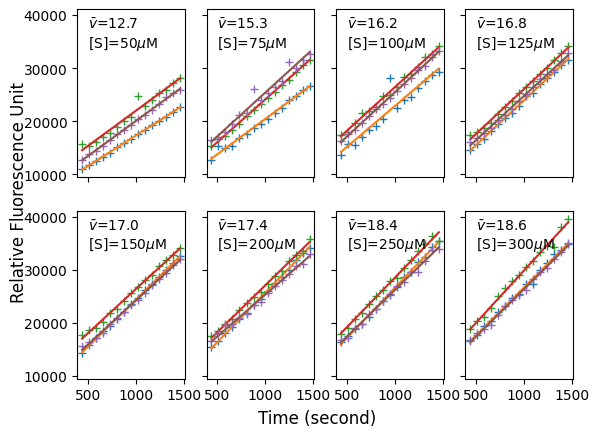
\includegraphics[width=1\linewidth]{../Figures/substrate1.png}
    \caption{Reaction Rate versus Substrate Concentration: 8 groups of experiments, each has 3 parallel groups}
    \label{Reaction Rate versus Substrate Concentration: 8 groups of experiments}
\end{figure}

\begin{figure}
    \centering
    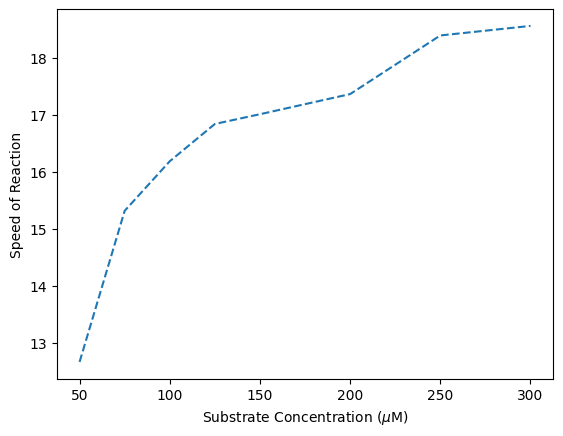
\includegraphics[width=1\linewidth]{../Figures/substrate2.png}
    \caption{Reaction Rate versus Substrate Concentration: in normal axes}
    \label{Reaction Rate versus Substrate Concentration: in normal axes}
\end{figure}

\begin{figure}
    \centering
    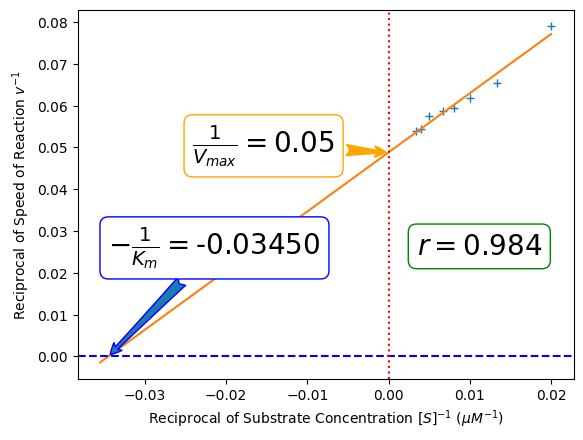
\includegraphics[width=1\linewidth]{../Figures/substrate3.png}
    \caption{Reaction Rate versus Substrate Concentration: in reciprocal axes}
    \label{Reaction Rate versus Substrate Concentration: in reciprocall axes}
\end{figure}


\section{Detecting Half-maximal Inhibitory Concentration}

\subsection{Introduction}
\begin{figure}
    \centering
    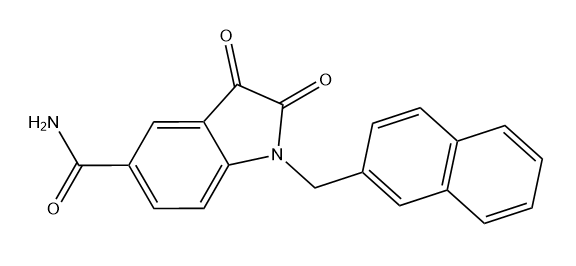
\includegraphics[width=0.7\linewidth]{../Figures/inhibitor structure.png}
    \caption{Structure of Inhibitor}
    \label{Structure of Inhibitor}
\end{figure}
The structure of inhibitor is shown in Figure \ref{Structure of Inhibitor}.
It will repress the reaction catalyzed by 3CL protease probably by competitive binding to the enzyme.
And we will determine the \textbf{Half-maximal Inhibitory Concentration, $IC_{50}$} through speed of reaction.



\subsection{Experimental Procedure}
The inhibitor is consist of competitive inhibitor, uncompetitive inhibitor and mixed inhibitor.
Instead of changing substrate concentration simultaneously, we varied inhibitor concentration [I] only and keep [S] under control.
Also, we focused on \textbf{Half-maximal Inhibitory Concentration ($IC_{50}$)} only, without concerns about modified factors to $V_{max}$ or $K_m$.

The following procedure was used to prepare to inhibitor solution with different concentration:

% List
\begin{itemize}
    \item sample 20 $\mu$L concentrated inhibitor(20 mM) solution with 180 $\mu$L DMSO as additional solvent. Then mix in $1^{st}$ well of microplate, which has the concentration of 200 $\mu$M.
    \item prepare 30 $\mu$L DMSO in each well of $1^{st}$ raw.
    \item take 30 $\mu$L solution from $1^{st}$ to $2^{nd}$ and mix in $2^{nd}$ well.
    \item repeat the step for the following wells to perform two fold serial dilution as shown in Figure \ref{Serial Dilution of Inhibitor}.
\end{itemize}

To get the solution of substrate, we decanted 1.92 mL DMSO into 2 mg fluorescent substrate then separated it into twelve different wells in the same row.
As shown in Figure \ref{Inhibitor Solution Configuration in Microplate}, the substrate and inhibitor were in different rows.
To be noted that, in reality, they were also stored in separated microplates to avoid unwanted illumination of fluorescent substrate.

The Composition of the System (100 $\mu$L):
\begin{itemize}
    \item Buffer Assay (80 $\mu$L, 80\%)
    \begin{itemize}
        \item \ce{Na2HPO4 / NaH2PO4} (40 mM)
        \item \ce{NaCl} (100mM)
        \item \ce{EDTA} (1mM)
        \item Triton X-100 (0.1\%)
    \end{itemize}
    \item SARS-CoV2-3CL Protease (10 $\mu$L, 10\%) (before mixing: 500 nM, after mixing: 50 nM)
    \item Fluorescent Substrate (5 $\mu$L, 5\%) (before mixing: 500 $\mu$M, after mixing: 25 $\mu$M)
    \item Inhibitor (5 $\mu$L, 5\%) (after mixing the serial concentration can be seen in Figure \ref{Reaction Rate versus Inhibitor Concentration: 12 groups of experiments, each has 3 parallel groups}).
    \item Temperature: 25$^\circ$C
\end{itemize}


\subsection{Data Analysis}
The reaction speed was also detected by \textbf{ELISA}.
Twelve subfigures are shown in Figure \ref{Reaction Rate versus Inhibitor Concentration: 12 groups of experiments, each has 3 parallel groups} and each of them corresponds to a different inhibitor concentration [I].
There are two intriguing phenomena in the figure.
Firstly, one group in [I]=10 $\mu$M and one group in [I]=1.25 $\mu$L exist extreme fluctuations which may caused by bubbles in solution.
Secondly, the reaction speed has negative value in high concentration of inhibitor.
The major cause of that absurd phenomenon is probably the unsteady state with fluctuation at early initial period.
To eliminate the negative value and disturbance of it, I also decided to omit the early four points, which should reasonable and appropriate.


\begin{figure}
    \centering
    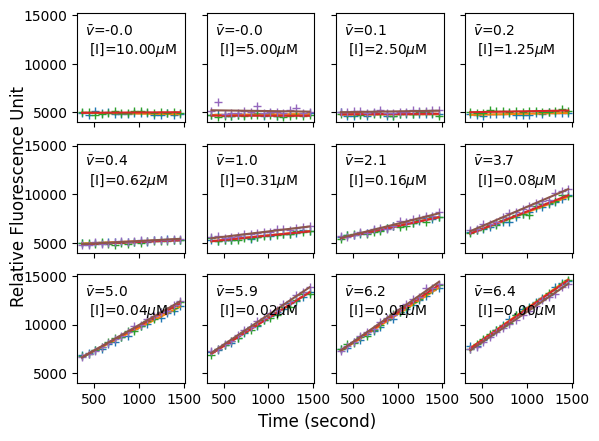
\includegraphics[width=1\linewidth]{../Figures/inhibitor1.png}
    \caption{Reaction Rate versus Inhibitor Concentration: 12 groups of experiments, each has 3
    parallel groups}
    \label{Reaction Rate versus Inhibitor Concentration: 12 groups of experiments, each has 3
    parallel groups}
\end{figure}

I performed linear regression again to each group and average the parallel groups to get the mean speed of reaction.
Then the plot of mean speed $\bar{V_0}$ versus inhibitor concentration was drawn.
From Figure \ref{Reaction Rate versus Inhibitor Concentration: determining IC50}, we can identify the \textbf{Half-maximal Inhibitory Concentration $IC_{50}$}, which is $IC_{50}=0.095\ \mu M$.
Somehow, the value is higher than the reported value $IC_{50}=0.095\ \mu M$.

$$
IC_{50}=0.095\ \mu \text{M}
$$

\begin{figure}
    \centering
    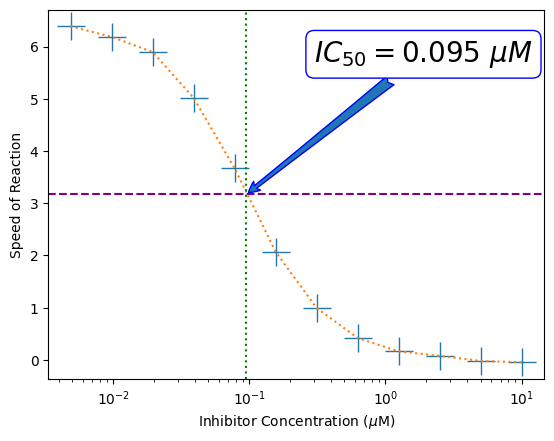
\includegraphics[width=1\linewidth]{../Figures/inhibitor2.png}
    \caption{Reaction Rate versus Inhibitor Concentration: determining IC50}
    \label{Reaction Rate versus Inhibitor Concentration: determining IC50}
\end{figure}

Besides, we can also figure out the inhibitory rate with different inhibitory concentration [I].
The intuitive recognition can be acquired in Figure \ref{Reaction Rate versus Inhibitor Concentration: determining IC50} while the precise values are shown in Table \ref{Inhibitory Rate with Different Inhibitor Concentration}.

\begin{table}
    \centering
    \caption{Inhibitory Rate with Different Inhibitor Concentration}

    \begin{tabular}{|c|c|c|}
        \toprule
         & Inhibitor Concentration ($\mu$M) & Inhibitory Rate \\
        \midrule
        0 & 10.00 & 100.00 \% \\
        1 & 5.00 & 99.59 \% \\
        2 & 2.50 & 98.07 \% \\
        3 & 1.25 & 96.72 \% \\
        4 & 0.62 & 92.77 \% \\
        5 & 0.31 & 83.84 \% \\
        6 & 0.16 & 67.12 \% \\
        7 & 0.08 & 42.29 \% \\
        8 & 0.04 & 21.31 \% \\
        9 & 0.02 & 7.65 \% \\
        10 & 0.01 & 3.15 \% \\
        11 & 0.00 & 0.00 \% \\
        \bottomrule
        \end{tabular}
    \label{Inhibitory Rate with Different Inhibitor Concentration}            
        
\end{table}

\bibliographystyle{plain}
\bibliography{references}

\end{document}